\chapter{Dinamica topologica Caotica}
Supponiamo che $X$ sia uno spazio metrico compatto e che $T:X\to X$ sia continua.
\section{Caos di Devaney}
\begin{definition}[Mappa topologicamente transitiva]
Sia $N$ spazio topologico e siano  $T:N\to N$ si dice \textbf{topologicamente transitiva} se per ogni coppia $U,V$ si aperti non vuoti esiste $n$ tale che $T^n(U)\cap V\neq \emptyset$.
\end{definition}
\begin{definition}[Dipendenza sensibile dalle condizioni iniziali]
Sia $N$ uno spazio metrico e $T:N\to N$ continua. $T$ ha \textbf{dipendenza sensibile dalle condizioni iniziali} su $N$ se esiste $c>0$ tale che per ogni $x\in N$ e per ogni $\e>0$ esiste $y\in B_\e(x)$ per cui esiste $n$ tale che $d(T^n(x),T^n(y))>c$.
\end{definition}
\begin{definition}[Caos di Devaney]
Affermiamo che $T$ \`e \textbf{caotica (nel senso di Devaney)} se esiste un sottoinsieme $\Lambda\subseteq X$ compatto e positivamente invariante tale che
\begin{enumerate}
\item l'insieme dei punti periodici \`e denso in $\Lambda$,
\item $T$ \`e topologicamente transitiva su $\Lambda$
\item $T$ ha dipendenza sensibile dalle condizioni iniziali su $\Lambda$.
\end{enumerate}
\end{definition}

\section{Entropia topologica}
\begin{definition}[Spazio $(n,\e)$-separato]
Sia $T:X\to X$ continua con $X$ metrico compatto. Dati $n\in\N$ e $\e>0$, un insieme $S\subseteq X$ \`e \textbf{$(n,\e)$-separato} se per ogni $x,y\in S$ distinti esiste $k\in\N$ con $k<n$ tale che $d(T^k(x),T^k(y))>\e$.
\end{definition}

\begin{definition}[Entropia topologica]
Sia $T:X\to X$ continua con $X$ metrico compatto. Definiamo l'\textbf{entropia topologica} di $T$ come
\[h_{top}(T)=\lim_{\e\to0^+}\limsup_{n\to+\infty}\frac1n\log\pa{\max\cpa{\# S\mid \text{$S$ \`e $(n,\e)$-separato}}}.\]
\end{definition}

\begin{definition}[Caos per entropia topologica]
Affermiamo che $T$ \`e \textbf{caotica (nel senso dell'entropia topologica)} se $h_{top}(T)>0$.
\end{definition}

\begin{proposition}[L'entropia topologica \`e invariante]\label{EntropiaTopologicaInvariantePerConiugioTopologico}
L'entropia topologica \`e invariante per coniugio topologico.
\end{proposition}
\begin{proof}
NON DATA DURANTE IL CORSO
\end{proof}

\begin{proposition}[Entropia topologica e partizioni]\label{EntropiaTopologicaEPartizioni}
Sia $T:[0,1]\to[0,1]$ tale che esiste $\Jc=\cpa{J_1,\cdots, J_k}$ partizione finita in intervalli tale che per ogni $i$ abbiamo $T(J_i)=[0,1]$ e $T\res{J_i}$ \`e invertibile e continua. Allora 
\[h_{top}(T)=\log k=\lim_{n\to+\infty}\frac1n\log(\#\cpa{Fix T^n}).\]
\end{proposition}
\begin{proof}[Dimostrazione (NON DATA DURANTE IL CORSO)]
	~
[QUESTA DIMOSTRAZIONE NON FUNZIONA, IGNORARE!!!]
Osserviamo che per ogni $n$, la partizione $\Jc=\Jc_1$ induce una partizione finita $\Jc_n$ pi\`u fine (composta da $k^n$ intervalli) data considerando gli intervalli dove $T^n$ \`e necessariamente invertibile e continua.
Senza perdita di generalit\`a supponiamo $\e<1/k$. In tal caso notiamo che $Fix T^n$ \`e un insieme $(n,\e)$-separato:\\
I punti di $Fix T^n$ appartengono a diversi intervalli di $\Jc_n$ e appartengono tutti alla parte interna di questi (altrimenti $T^n\res{int(J^{(n)}_j)}$ non potrebbe essere invertibile). Siano $x,y\in Fix T^n$ punti distinti e sia $k$ il pi\`u piccolo intero tale che $y$ e $x$ appartengono ad intervalli diversi per la partizione $\Jc_k$. Notiamo che $k$ esiste ed \`e compreso tra $1$ e $n$ per costruzione. [QUESTO PEZZO NON FUNZIONA] Affermiamo che $d(T^k(x),T^k(y))>1/k>\e$, infatti per costruzione delle partizioni $T^k(x)$ e $T^k(y)$ appartengono ad elementi diversi di $\Jc$ e quindi per ipotesi su $\e$ distano pi\`u di $\e$.

Osserviamo che se $\e>1/m$ allora la massima cardinalit\`a di un insieme $(0,\e)$-separato \`e $m$. Un insieme $S$ $(n,\e)$-separato di massima cardinalit\`a possibile pu\`o perci\`o contenere al massimo $k^nm$ punti in quanto ogni punto deve distare da ogni altro punto almeno $\e$ applicando una mappa della forma $T^r$ per qualche $r\leq n$\footnote{il miglior caso \`e porre avere $m$ punti in ogni elemenento di $\Jc_n$.}. Si ha dunque che 
\begin{align*}
h_{top}(T)\leq&\lim_{m\to+\infty}\lim_{\e\to\frac1m^+}\limsup_{n\to+\infty}\frac1n\log\pa{k^nm}=\\
=&\log k +\lim_{m\to+\infty}\lim_{\e\to\frac1m^+}\under{=0}{\limsup_{n\to+\infty}\frac{\log m}n}=\log k.
\end{align*}
Abbiamo dunque mostrato che $\log k\leq h_{top}(T)$ e $h_{top}(T)\leq \log k$ come voluto.
\end{proof}

\begin{proposition}[Entropia di una rotazione]
Sia $T_\al:S^1\to S^1$ dato da $T_\al(x)=x+\al\mod 1$. Allora $h_{top}(T_\al)=0$
\end{proposition}
\begin{proof}[Dimostrazione. (Esercizio)]
Notiamo che $T_\al$ \`e una isometria, quindi $d(T_\al^k(x),T^k_\al(y))>\e$ se e solo se $d(x,y)>\e$. Segue che un insieme \`e $(n,\e)$-separato se e solo se \`e $(0,\e)$-separato. La massima cardinalit\`a di un tale insieme \`e $\floor{\e\ii}$, che in particolare \`e un valore costante in $n$. Segue dunque che
\[h_{top}(T)=\lim_{\e\to0^+}\limsup_{n\to+\infty}\frac1n\log(\floor{\e\ii})=\lim_{\e\to0^+}0=0.\]
\end{proof}

\section{Ferro di cavallo}
\begin{definition}[Ferro di cavallo]
Una funzione continua $T:[a,b]\to[a,b]$ ha un \textbf{ferro di cavallo} se esiste $J\subseteq [a,b]$ intervallo chiuso che ricopre se stesso almeno due volte.
\end{definition}

\begin{proposition}[Relazione tra ferro di cavallo e periodi minimi]\label{RelazioneFerroDiCavalloEPeriodiMinimi}
Sia $T:[a,b]\to[a,b]$ continua.
\begin{enumerate}
\item Se $T$ ha un ferro di cavallo allora ammette orbite per ogni periodo minimo.
\item Se $T$ ammette un'orbita di periodo minimo $m$ dispari allora $T^2$ ha un ferro di cavallo. 
\end{enumerate}
\end{proposition}
\begin{proof}
Mostriamo i due punti
\setlength{\leftmargini}{0cm}
\begin{enumerate}
\item Per il teorema di Sharkovsky (\ref{TeoremaSharkovsky}) basta il periodo minimo 3.\\ 
Per definizione di ferro di cavallo esistono $K_1$ e $K_2$ intervalli aperti disgiunti tali che $T(\ol K_i)=J$ per un opportuno intervallo $J$ di $[a,b]$. Se $\ol K_1\cap \ol K_2=\cpa{z}$ con $z$ punto fisso allora osserviamo graficamente che esiste $\ol K_3\subseteq \ol K_1$ tale che $\ol K_3\cap \ol K_2=\emptyset$ e $K_2$ e $K_3$ coprono $J$. Quindi sostituiamo $K_1$ con $K_3$.

\begin{figure}[!htb]
	\centering
	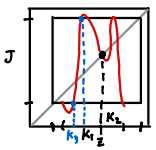
\includegraphics[width=3cm]{Immagini/esempio_Dimostrazione_ferro_di_cavallo.png}
\end{figure}

Definiamo una partizione di $[a,b]$ che contenga $\ol K_1$ e $\ol K_2$. Cos\`i facendo avremo un $T$-grafo dove $\ol K_1\ol K_2\ol K_2\ol K_1$ \`e ammissibile. Per il teorema (\ref{CriterioTGrafoPerEsistenzaOrbitePeriodiche}) esiste $x\in K_1$ tale che $T^3(x)=x$ e $T(x)\in \ol K_2$. Chiaramente $x$ ha periodo minimo 1 o 3, ma se $T(x)=x$ allora $\ol K_1\cap \ol K_2=\cpa{x}$ sarebbe un punto fisso, contraddicendo le ipotesi.
\item Supponiamo senza perdita di generalit\`a che $m$ sia minimo. Fissiamo un'orbita con periodo minimo $m$ e ordiniamo i vertici secondo la configurazione trovata dimostrando (\ref{TeoremaSharkovsky})\footnote{Figura \ref{ConfigurazioneOrbita}. In questa configurazione $J_{\ol h}=I_1=[P_1,P_2]$. Se la configurazione fosse la simmetrica rispetto a quella in figura nella notazione seguente vanno scambianti gli estremi degli intervalli }. Notiamo che esiste $x_0$ fisso in $[P_1,P_2]$ e $y_0\in [P_{m},P_{m-2}]$ tale che $T(y_0)=x_0$. Applicando un po' di volte il teorema del valore intermedio come in figura 

\begin{figure}[!htb]
	\centering
	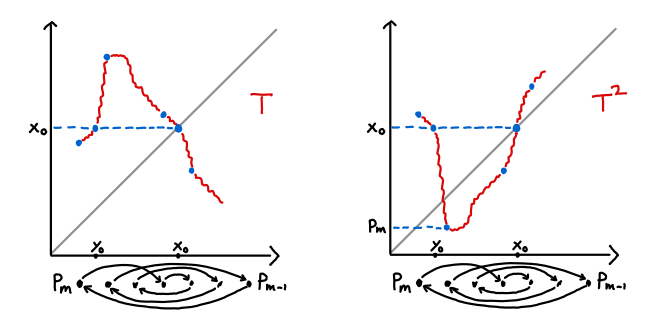
\includegraphics[width=8cm]{Immagini/Ferro_cavallo_2.png}
\end{figure}

osserviamo che $J=[P_m,x_0]$ copre se stesso almeno due volte per $T^2$ \footnote{infatti $[P_m,x_0]\subseteq T([y_0,P_{m-2}])\cap T([P_{m-2},x_0])$.}.
\end{enumerate}
\setlength{\leftmargini}{0.5cm}
\end{proof}

\section*{Equivalenza tra le definizioni}
\begin{theorem}[Caratterizzazione del Caos]\label{CaratterizzazioneCaos}
Sia $T:[a,b]\to [a,b]$ continua. Allora le seguenti sono affermazioni sono equivalenti:
\begin{enumerate}
\item $T$ \`e caotica nel senso di Devaney
\item $h_{top}(T)>0$
\item Esiste $n\in\N$ per cui $T^n$ ha un ferro di cavallo
\item esiste orbita periodica per $T$ di periodo minimo $m$ non potenza di $2$.
\end{enumerate}
\end{theorem}
\begin{proof}
L'equivalenza tra le ultime due \`e la proposizione (\ref{RelazioneFerroDiCavalloEPeriodiMinimi}). Per il resto la dimostrazione non \`e stata data durante il corso.
\end{proof}

